\documentclass[11pt, oneside, a4paper]{article}
%\documentclass[11pt, oneside, a4paper, twocolumn]{article}
\usepackage[utf8]{inputenc}
\edef\restoreparindent{\parindent=\the\parindent\relax}
\usepackage{parskip}
\restoreparindent
\usepackage{indentfirst}
\setlength{\topmargin}{-1in}
\setlength{\textheight}{10.2in}
\setlength{\textwidth}{7.1in} 
\setlength{\footskip}{0.6in}
\setlength{\oddsidemargin}{-0.3in}
\pretolerance=150
\newcommand{\cm}[1]{\par\textbf{{#1}}\par}
\usepackage[ backend=bibtex, natbib=true, style=numeric, sorting=none]{biblatex}
\addbibresource{library.bib}

\usepackage{csquotes}
\usepackage[svgnames]{xcolor}
\usepackage[colorlinks=true, citecolor=Black, linkcolor=Black, urlcolor=Black]{hyperref}
\usepackage{bookmark}
\usepackage{mathtools}
\usepackage{float}
\usepackage{subcaption}
\usepackage{svg}
%\setsvg{inkscapeexe=dbus-run-session, inkscapeopt=inkscape}
\usepackage{algorithm2e}
\begin{document}
\title{Biological Tissue Movement}
\author{Oleksandr Hubanov\\
Vilnius Gediminas Technical University}
\maketitle
\chapter*{Introduction}
%Введение и постановка задачи 
The mitral valve, also known as the bicuspid valve or left atrioventricular
valve, is a valve with two flaps in the heart, that lies between the left atrium
and the left ventricle. The mitral valve and the tricuspid valve are known
collectively as the atrioventricular valves because they lie between the atria
and the ventricles of the heart.
\begin{figure}[H]
  \centering
  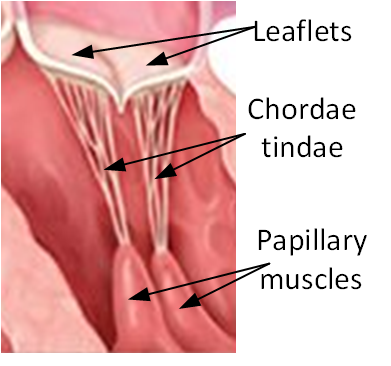
\includegraphics[width=0.4\textwidth]{./fig/mt.png}
    \caption{Mitral valve structure}
    \label{fig:MT}
\end{figure}
Mechanical properties
Chordae:
L ~ 0,025 m (length)
d ~ 0,001 m (diameter)
$\rho$ = 1040 kg/m3 (density)
E = 2000 N/m (stiffness)
Poisson's ratio of 0.49

Leaflets:
E = 2.0E6 MPa (Anterior leaflet)
E = 1.0E6 MPa (Posterior leaflet)
$\rho$ = 1.06E3 kg/m3 
Poisson’s ratio 0.49 
\par
Mitral valve has cyclic working conditions. Example of such you can see on
figure \ref{fig:workMT}.
\begin{figure}[H]
  \centering
  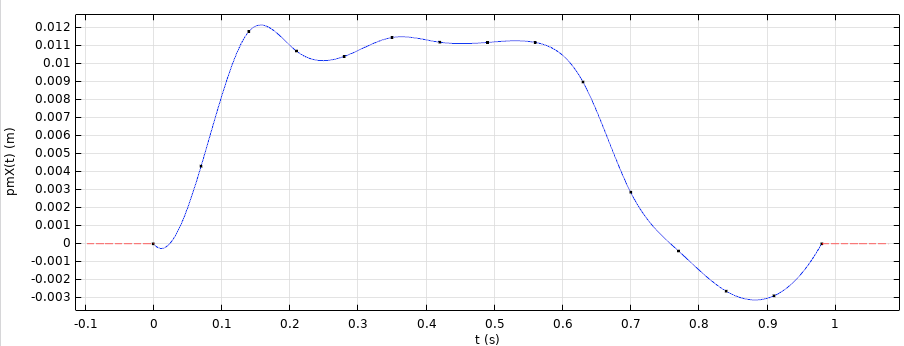
\includegraphics[width=0.8\textwidth]{./fig/workMT.png}
    \caption{Displacement of papillary muscle over cardiac cycle}
    \label{fig:workMT}
\end{figure}
 In normal conditions, blood flows through an open mitral valve during diastole
with contraction of the left atrium, and the mitral valve closes during systole
with contraction of the left ventricle. The valve opens and closes because of
pressure differences, opening when there is greater pressure in the left atrium
than ventricle, and closing when there is greater pressure in the ventricle than
atrium. In abnormal conditions, blood may flow backwards through the valve
(mitral regurgitation) or the mitral valve may be narrowed (mitral stenosis).
Rheumatic heart disease often affects the mitral valve; the valve may also
prolapse with age, and be affected by infective endocarditis. The mitral valve
is named after the mitre of a bishop, which resembles its flaps.
\begin{figure}[H]\label{fig:workingMT}      
  \centering
  \begin{subfigure}[b]{0.4\textwidth}\label{fig:openMT}
    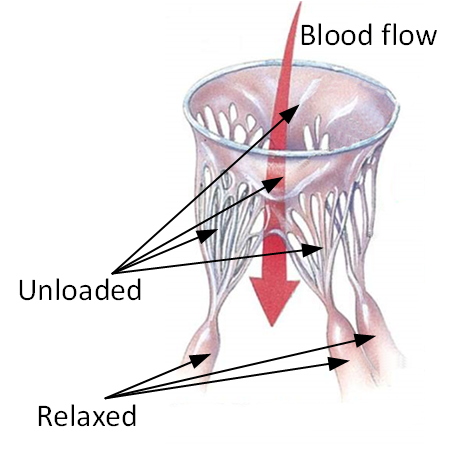
\includegraphics[width=\textwidth]{./fig/openMT.png}
      \caption{Opened state of mitral valve}      
  \end{subfigure}
  ~
  ~ %add desired spacing between images, e. g. ~, \quad, \qquad, \hfill etc. 
    %(or a blank line to force the subfigure onto a new line)
  \begin{subfigure}[b]{0.4\textwidth}\label{fig:closedMT}  
    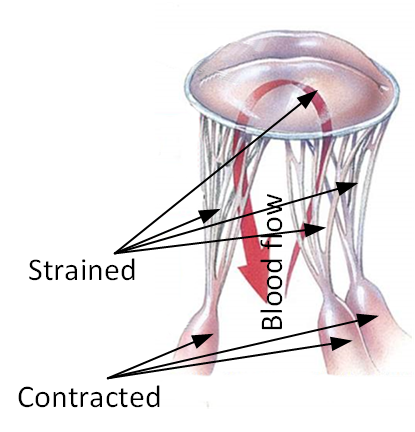
\includegraphics[width=\textwidth]{./fig/closedMT.png}
      \caption{Closed state of mitral valve}    
  \end{subfigure}
  \caption{Mitral valve working cycle}
\end{figure} 

Mitral valve prolapse (MVP) is a valvular heart disease characterized by the
displacement of an abnormally thickened mitral valve leaflet into the left
atrium during systole. By other words, it is a condition in which the two flaps
of the mitral valve doesn't close smoothly and evenly, but instead bulge
(prolapse) upward into the left atrium.\cite{Hayek2005a}
\begin{figure}[H]\label{fig:compareMT}
  \centering
  \begin{subfigure}[b]{0.4\textwidth}\label{fig:normalMT}
    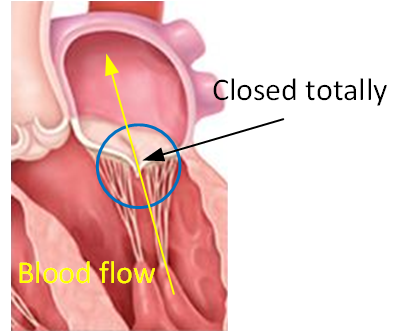
\includegraphics[width=\textwidth]{./fig/normalMT.png}
      \caption{Normal mitral valve}      
  \end{subfigure}
  ~
  ~ 
  \begin{subfigure}[b]{0.4\textwidth}\label{fig:prolapseMT}
    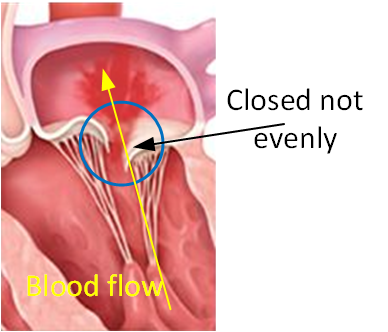
\includegraphics[width=\textwidth]{./fig/prolapseMT.png}
      \caption{Prolapse mitral valve}      
  \end{subfigure}
  \caption{Comparison of the normal valve and prolapse}      
\end{figure} 
Providing the surgeon with an anatomically and biomechanically accurate
computional model of a particular patient's mitral heart valve could enable
preoperative surgical planning and potentially improve surgical outcome.
Investigation behavior of biological tissue can be done by estimating movement
of it. Tissues of biological origin, usually had a weak structure and little
stiffness.
\par
%FEM explisit(abaqus) and MSM
Such physical structure imposes restrictions on the possible tools in the
measurement. Another possible problem is the limited number of measurement
attempts. Such limitations of physical measurements call into question the
possibility of such activities in general. An alternative to physical
experiments is the numerical simulation of these experiments. There are a large
number of different numerical modeling methods. All of them are derivatives of
Finite Element Method(FEM) and Discrete Element Method(DEM).
\par
While general finite-element studies are helpful for the evaluation and
development of MV repair surgery, patient-specific models are required for
individual therapy planning.
\cm{article 1}
The patient-specific mass-spring MV model uses a segmentation of 3D TEE images
for the initialization of a mass-spring model of the closed MV under systolic
pressure. An iterative approach is used to adjust the spring rest-length so that
the model can accurately simulate the shape of the closed MV under systolic
pressure. To simulate MV annuloplasty, the model can then be deformed, according
to the annuloplasty ring to be used, to create a prediction of the shape of the
closed MV after surgery.
\par
Based on the properties of the material of biological tissues and review of
existing projects, the most appropriate method is Mass - Spring modeling(MSM). This
method based on ideas of DEM and basic element here is very know in mechanic
simple one dimensional(1D) beam.\ref{eqn:sacdd}
\cm{have to show so pic about MSM, with explanation what is going on}
Computational complexity of MSM is much less compare to FEM-based methods,
because of less number of equations to integrate on each time step. This
important advantage and physics way have method describes basic element gave to
MSM very wide using in computer games for calculating reality-looks hair or
cloth movement in real time. Modelling by using MSM could be parallel calculated
on each time step.\cite{Rasmusson2008} \cite{Amorim2012}
\par
%В расчете целого клапана берется один стержень, существующие варианты расчетов всей системы и как в них рассчитывается хорда
\begin{figure}[H]\label{fig:pc1}
  \centering
  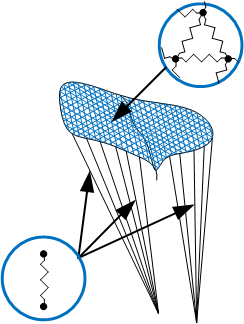
\includegraphics[width=0.2\textwidth]{./fig/pc1.png}
    \caption{Displacement of papillary muscle over cardiac cycle}    
\end{figure}
\begin{figure}[H]\label{fig:pc2}
  \centering
  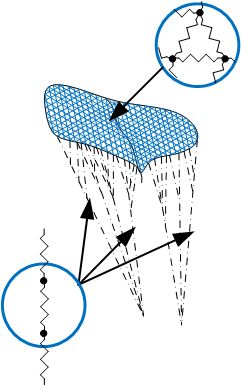
\includegraphics[width=0.2\textwidth]{./fig/pc2.png}
    \caption{Displacement of papillary muscle over cardiac cycle}    
\end{figure}
\begin{figure}[H]\label{fig:pc3}
  \centering
  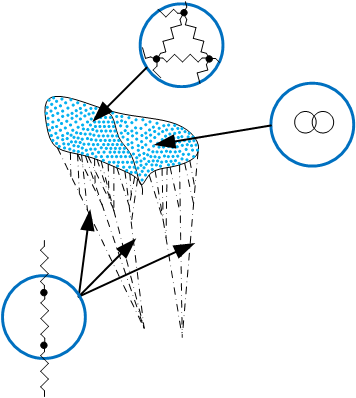
\includegraphics[width=0.3\textwidth]{./fig/pc3.png}
    \caption{Displacement of papillary muscle over cardiac cycle}    
\end{figure}
%Как движется кровь, описать механику (давление и скорость) сравнить преимущ от расчета давления от скорости
%Цель- сравнить одну стержень и систему
\section*{Mathematical model}
~\par
%Хорда описана ломаной линией из элементов первого порядка, 
Fibrous tissue could be described as system of 1D rods, in case of getting mechanical 
equivalent of system.
Example of such flat 2D system are shown on figure \ref{fig:nodeExtract}.
\begin{figure}[H]\label{fig:rodSystem}
  \centering
  \includesvg[width=0.8\columnwidth]{fig/systemAtworld}
  \caption{1D Rod system in global coordinate system}
\end{figure}
System consists of discrete elements $e_1$, $e_2$ and $e_3$. All elements are
connected to each other through nodes $n_2$, $n_3$ and to special points through
$n_1$ and $n_4$. Each element $e_n$ of system has own orientation in global
coordinate system. 
From schematic representation of node comes that all vector variables of node should be calculated
in global coordinate system and element variables in own local coordinate system(figure
\ref{fig:nodeExtract}). For transformation between coordinate systems direction cosine matrix
(DCM)\eqref{eqn:DCM} can be used.
\begin{equation}\label{eqn:DCM}
  DCM= \begin{bmatrix}
    cos(X,x) & cos(X,y) & cos(X,z) \\
    cos(Y,x) & cos(Y,y) & cos(Y,z) \\
    cos(Z,x) & cos(Z,y) & cos(Z,z) \\
  \end{bmatrix}
\end{equation}
where $\{X, Y, Z\}$ is global coordinate system and $\{x,y,z\}$ is local coordinate
system.\par According to primitive scheme of node \ref{fig:nodeExtract}, mass of
each node can be calculated, like sum of half mass of each element, which acting
in node. $m_n=\sum_{e}m_e/2$\par
In case that node does not have external interrupt, like pressure or other
applied force, schematic represent of node can be as on figure
\ref{fig:nodeExtract}.\par
\begin{figure}[H]
  \centering
  \includesvg[width=0.6\columnwidth]{fig/nodeExtract}
  \caption{Extracted node from system}\label{fig:nodeExtract}
\end{figure}
Mathematical model of discrete system is expressed by equations of nodes motion.
All system acting in global coordinate system $\{X, Y, Z\}$ and each element acting
in own local coordinate system $\{x,y,z\}$.
%FEM explisit(abaqus) and MSM
Such physical structure imposes restrictions on the possible tools in the
measurement. Another possible problem is the limited number of measurement
attempts. Such limitations of physical measurements call into question the
possibility of such activities in general. An alternative to physical
experiments is the numerical simulation of these experiments. There are a large
number of different numerical modeling methods. All of them are derivatives of
Finite Element Method(FEM) and Discrete Element Method(DEM).\par
While general finite-element studies are helpful for the evaluation and
development of MV repair surgery, patient-specific models are required for
individual therapy planning.
The patient-specific mass-spring MV model uses a segmentation of 3D TEE images
for the initialization of a mass-spring model of the closed MV under systolic
pressure. An iterative approach is used to adjust the spring rest-length so that
the model can accurately simulate the shape of the closed MV under systolic
pressure. To simulate MV annuloplasty, the model can then be deformed, according
to the annuloplasty ring to be used, to create a prediction of the shape of the
closed MV after surgery.\par
Based on the properties of the material of biological tissues and review of
existing projects, the most appropriate method is Mass - Spring modeling(MSM). This
method based on ideas of DEM and basic element here is very know in mechanic
simple one dimensional(1D) beam.
\cm{have to show so pic about MSM, with explanation what is going on}
Computational complexity of MSM is much less compare to FEM-based methods,
because of less number of equations to integrate on each time step. This
important advantage and physics way have method describes basic element gave to
MSM very wide using in computer games for calculating reality-looks hair or
cloth movement in real time. Modelling by using MSM could be parallel calculated
on each time step.\cite{Rasmusson2008} \cite{Amorim2012}\par
%В расчете целого клапана берется один стержень, существующие варианты расчетов всей системы и как в них рассчитывается хорда
\begin{figure}[H]\label{fig:pc1}
  \centering
  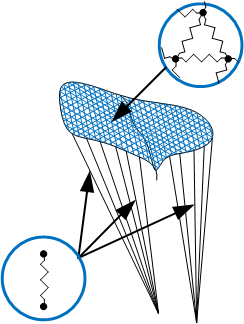
\includegraphics[width=0.35\columnwidth]{./fig/pc1.png}
  \caption{Displacement of papillary muscle over cardiac cycle}
\end{figure}
\begin{figure}[H]\label{fig:pc2}
  \centering
  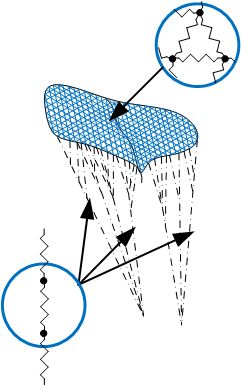
\includegraphics[width=0.35\columnwidth]{./fig/pc2.png}
  \caption{Displacement of papillary muscle over cardiac cycle}
\end{figure}
\begin{figure}[H]\label{fig:pc3}
  \centering
  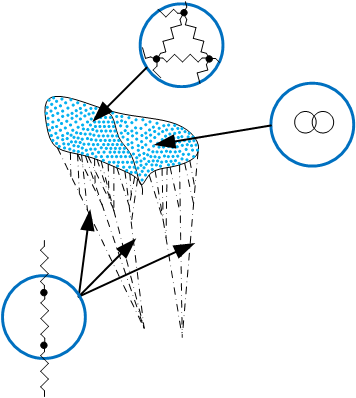
\includegraphics[width=0.45\columnwidth]{./fig/pc3.png}
  \caption{Displacement of papillary muscle over cardiac cycle}
\end{figure}
\cm{research aim is to compare 1 rod and rope of rods}
%Понятие линейной деформации, допущения, понятия и эфекты
%Движение узлов 
%Описать силы в узлах от стержней
%Учет напрвления элементов
\section*{Mass Spring Model}
\subsection*{Linear deformation}
For investigating motion of any mechanical system need to integrate equation of
motion\eqref{eqn:motionEq}. For this propose need to express all acting forces in
node\eqref{eqn:sumF} for each node in relation to their application place. 
\begin{equation}\label{eqn:sumF}
   \vec{F}_n= \vec{F}_{ext} + \sum\vec{F}_{elem}\times[DCM] + \vec{F}_{press}\times[DCM]
\end{equation}\par
$F_{ext}$ is external load force, applied to node in global coordinates. Value of this force for
each time step is loaded from list of loads.\par $F_{press}$ is external pressure and can be
described like force applied to element in local coordinates.\par $F_{elem}$ is sum of internal
forces of each element, which acting in node. From each element counts only half of force to node,
other half going to neighbour node. In case of 1D element system, internal force of each element can
be express like axial force and it is equal to integral of stress over area:
\begin{equation}\label{eqn:Nx}
  N(x)= \int\limits_A \sigma dA
\end{equation}
For 1D rod system $F_{elem}$ can be expressed like:
\cm{Is it has to be divided by 2? in this case how to calc mass of node?}
\begin{equation}\label{eqn:Felem}
  F_{elem} = \sum_{e}N_e(x)/2
\end{equation}\par
The motion of nodes can be expressed by Newton's equation of motion\ref{eqn:motionEq}. As 1D
element was choosed as discrete element, only the normal component of the
translational motion is considered, the equation reduces to\par
\begin{equation}\label{eqn:motionEq}
  m\vec{\ddot{x}} + k\vec{x} + c\vec{\dot{x}} = \vec{F_n}
\end{equation}
where $F_n$ is force acting in node $n$, $m$ – mass of node and $\ddot{x}$ is acceleration, $k$ –
stiffness coefficient of node, $x$ is displacement of node and $c$ – damping coefficient of node,
$\dot{x}$ is velosity of node, initial conditions are: $x(0)=0$ and $\dot{x}(0)=V_0$. According to
\ref{eqn:sumF}, $kx$ are described by $\sum{F_{elem}}$, $c\dot{x}$ are described by $F_{press}$ and
motion equantion will become to:
\begin{equation}\label{eqn:motionEqNodeStatic}
  \vec{F}_{press} + \sum{F_{elem}} + m\vec{\ddot{x}} = \vec{F}_n
\end{equation}
where $F_{elem}$ is sum of node's elements forces, $m$ – mass of node and $\ddot{x}$ is
acceleration. In static case $m\ddot{x}$ equal to zero, due zero acceleration, because no external
force is applied and equantion of node is balansed. But if external force are applied, motion will
start, motion equation will become not balansed\ref{eqn:motionEqDynamic}, mass start to act as inertia. 
\begin{equation}\label{eqn:motionEqDynamic}
  \vec{F}_{press} + \sum\vec{F}_{elem} + m\vec{\ddot{x}} = F_n + \vec{F}_{ext}
\end{equation}\par 
Equations of motion for Euler's scheme of integration can be described like:
\begin{equation}\label{eqn:Accel}
  \vec{\ddot{x}}(t +\Delta t)=\vec{F}_n/m
\end{equation}
\begin{equation}\label{eqn:Velos}
  \vec{\dot{x}}(t +\Delta t)=\vec{\dot{x}}(t)+\vec{\ddot{x}}(t)\Delta t
\end{equation}
\begin{equation}\label{eqn:Displ}
  \vec{x}(t +\Delta t)=\vec{x}(t)+\vec{\dot{x}}(t)\Delta t
\end{equation}
\par Element force becomes from physical deformation of
element. In linear case of study, deformation of element much less compare to
element dimensions. It is expressed by linear geometry
equation\eqref{eqn:linDeformation}, which showing relation between initial
length of element and length in $\Delta t$ state.
\begin{equation}\label{eqn:linDeformation}
  \varepsilon=\frac{dU}{dx}=\frac{l(\Delta t)-l(t)}{l(t)}
\end{equation}
According to Hook law $\sigma=\varepsilon E$ and linear geometry equation
\eqref{eqn:linDeformation}, inner force can be described as:
\begin{equation}\label{eqn:linNxFull}
  N(x)= \int\limits_{Al} \varepsilon EdldA=EA\int\limits_l \varepsilon dl=\frac{EA}{l(t)}*(l(t + \Delta t)-l(t))
\end{equation}
where $l(\Delta t)$ is current length of element, $l(t)$ length of element at previuous time moment,
$E$ – Young’s modulus for element material, $A$ – volume of element. To be able to integrate
equation of motion, need to express deformation in equation \eqref{eqn:linNxFull} by differences
between displacements of nodes, to which element is connected:
\begin{equation}\label{eqn:linNxWdispl}
  N(x)=\frac{EA}{l(t)}*(x_{i}(t)-x_{j}(t))
\end{equation}\par
%Нелинейное деформ стержня, по времени
%Описать допущение что модуль упрогости = нелинейность
%\subsection*{Nonlinear deformation}
%Nonlinearity in main mean that element can get huge deformation compare to
%element demesions. Equation of $F_{elem}$ in this case  would change to
%nonlinear form:
%\begin{equation}\label{eqn:nonlinNx}
%  N(x)= \int\limits_t\int\limits_A \sigma dAdt
%\end{equation}
%From this equantion comes that cross sectional area and stiffness coefficient
%will get nonlinearity.
% \par
%Changing of cross sectional area over time for 1D element is changing its length
%over time. Linear geometry equation\eqref{eqn:linDeformation}, showing linear
%relations between length, because difference in $\Delta t$ state takes according
%initial length of element. In case of huge deformation need to recalculate
%length of element on each time step and take difference of displacement
%according to previous time step. In end of geometry equation become to nonlinear
%form:
%\begin{equation}\label{eqn:nonlinDeformation}
%  \varepsilon=\frac{dU}{dx}=\frac{l(\Delta t)-l(t-\Delta t)}{l(\Delta t)}
%\end{equation}
%Inner force\eqref{eqn:linNxFull} also become to nonlinear form:
%\begin{equation}\label{eqn:nonlinNxFull}
%  N(x)= \int\limits_t\int\limits_A \varepsilon EdA=EA\int\limits_t\varepsilon=\frac{EA}{l(\Delta t)}*(l(\Delta t)-l(t-\Delta t))
%\end{equation}
%where $l$ is current length of element, $l_0$ length of element at $t=0$, $E$ –
%Young’s modulus for element material.\par And nonlinear equantion of inner force
%for integration:
%\begin{equation}\label{eqn:nonlinNxWdispl}
%  N(x)=\frac{EA}{l_0}*(U_{i}-U_{j})
%\end{equation}\par

\par
Let's try to describe minimal possible way to get simulation of such structure
 as shown on figure \ref{fig:rodSystem}. 

\begin{algorithm}[H]\label{algo:calcNodeMovement}
  initialization\;
  \tcp{Preform integration nodes movement over time}
  \tcp{Initial state is $x(0)=\dot{x}(0)=\ddot{x}(0)=0$}
  \tcp{Iterate over time}
  \While{$t < t_{end} - 1$}{
    \tcp{Iterate over nodes}
    \ForEach{node in nodes}
    {
      \tcp{get external force loading}
      $F_{ext}$ = getFext(node, t)\;
      \tcp{push $F_{ext}$ into current node force $F_n$}
      $F_n$ = $F_n + F_{ext}$\;
      \tcp{calc $F_{elm}$ from previous displacement}
      \ForEach{link in neighbours}
      {
        $F_{elm}$ = getFelm(node, link)\;
        \tcp{convert $F_{elm}$ from local to global coordinates}
        $F_{elm}G$ = $F_{elm}\times[DCM]$\;
        \tcp{push $F_{elm}G$ into current node force $F_n$}
        $F_n$ = $F_n + F_{elm}G$\;
      }
      \tcp{calc pressure force}
      $F_{press}$ = getFpress(node, t)\;
      \tcp{convert $F_{elm}$ from local to global coordinates}
      $F_{press}G$ = $F_{press}\times[DCM]$\;
      \tcp{push $F_{elm}G$ into current node force $F_n$}
      $F_n$ = $F_n + F_{press}G$\;
      \tcp{integrate collected $F_n$ to get derivatives of $x$ for $t + \Delta t$}
      $[x(t + \Delta t), \dot{x}(t + \Delta t), \ddot{x}(t+ \Delta t)]$ = integrate($F_n, x(t), \dot{x}(t), \ddot{x}(t)$ )
    }
  }
 \end{algorithm}
  
\newpage
%Движение в жидкости
%Как движется кровь, описать механику (давление и скорость) 
%сравнить преимущ от расчета давления от скорости

\section*{Integration schemes}

\section*{Results}

\printbibliography[title=List of literature]
\end{document}
